\section{Utilizzo}

\subsection{Amministratore}



\subsection{Dipendente}

\subsubsection{Login}
\begin{figure}[H]
	\centering
	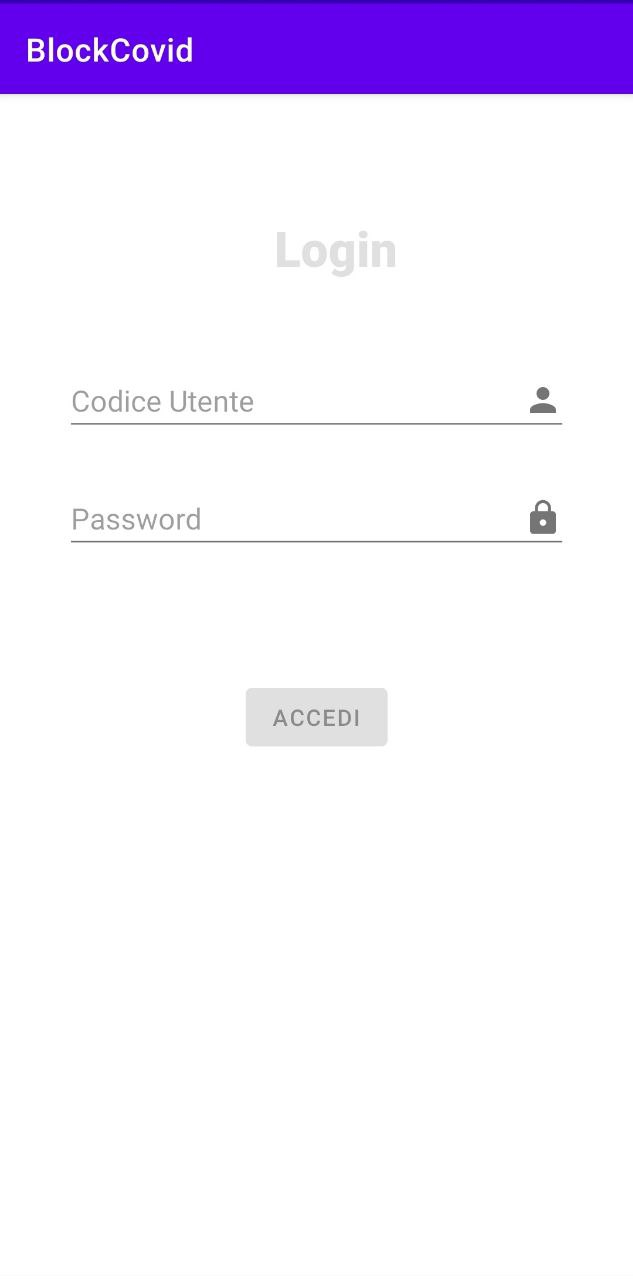
\includegraphics[width=5cm]{res/images/login.png}
	\caption{Login utente}
\end{figure}
L'utente può autenticarsi inserendo il proprio username e la propria password. 

\subsubsection{Logout}
\begin{figure}[H]
	\centering
	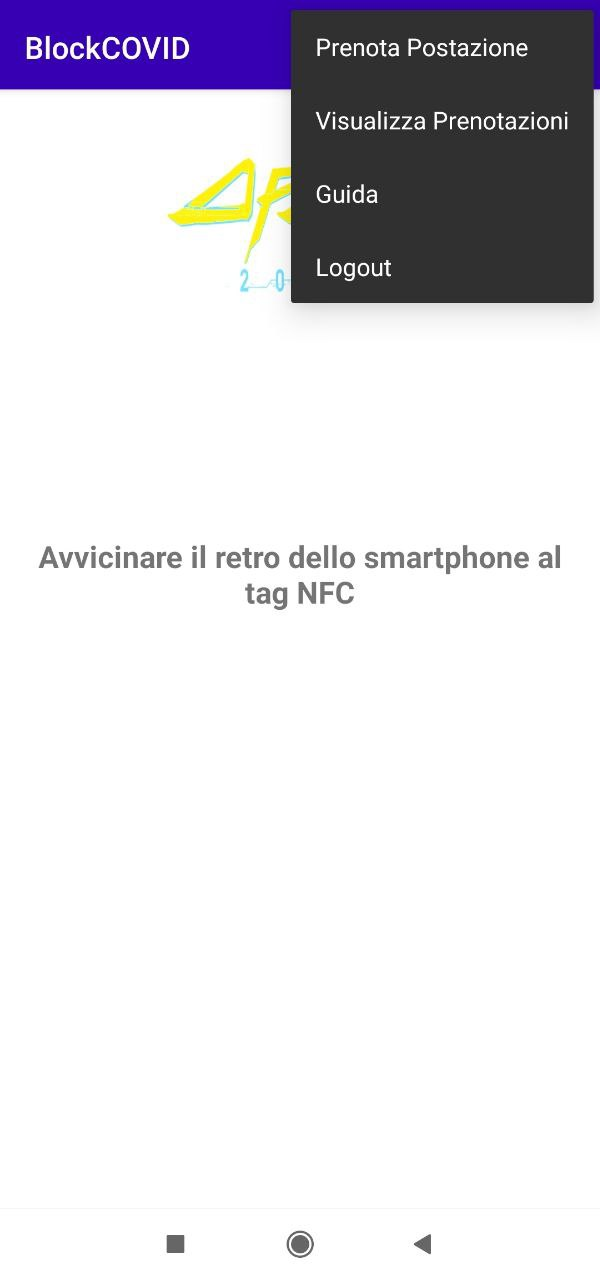
\includegraphics[width=5cm]{res/images/menuATendina.png}
	\caption{Logout utente}
\end{figure}
L'utente può eseguire il logout aprendo il menù a tendina e poi cliccando su Logout.

\subsubsection{Scansione tag NFC}
\begin{figure}[H]
	\centering
	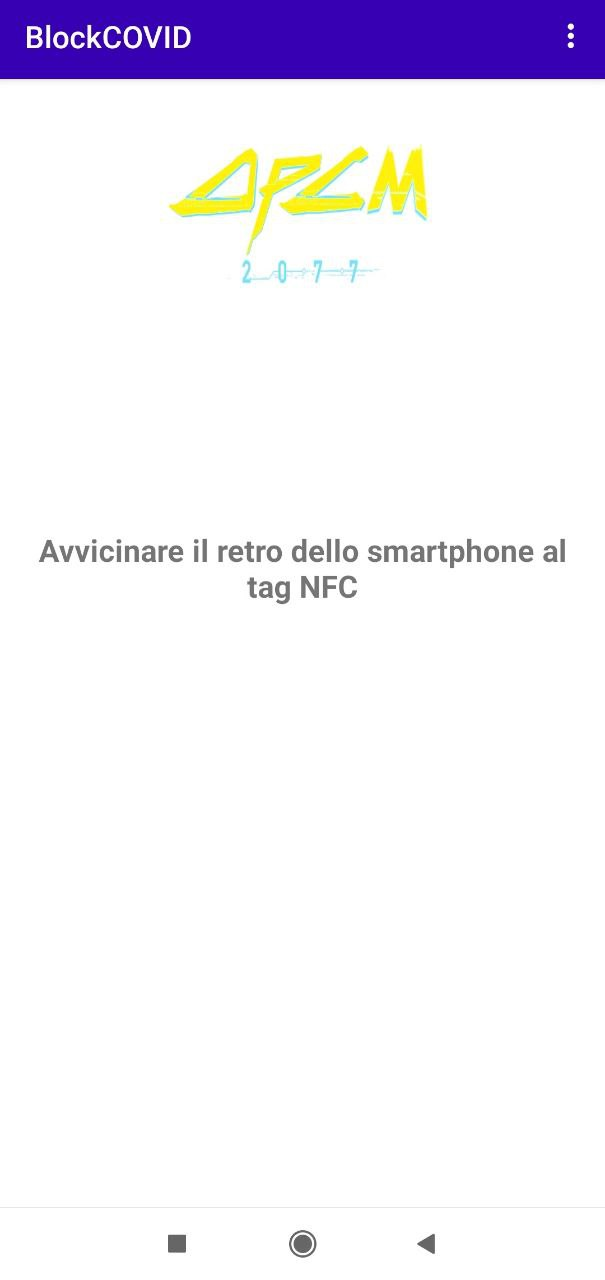
\includegraphics[width=5cm]{res/images/avvicinaSmartphone.png}
	\caption{Scansione tagNFC}
\end{figure}
L'utente si trova nella pagina principale dell'applicazione e gli viene chiesto di effettuare una scansione del tag NFC tramite lo smartphone. 
\subsubsection{Visualizzazione stato postazione}
\begin{figure}[H]
	\centering
	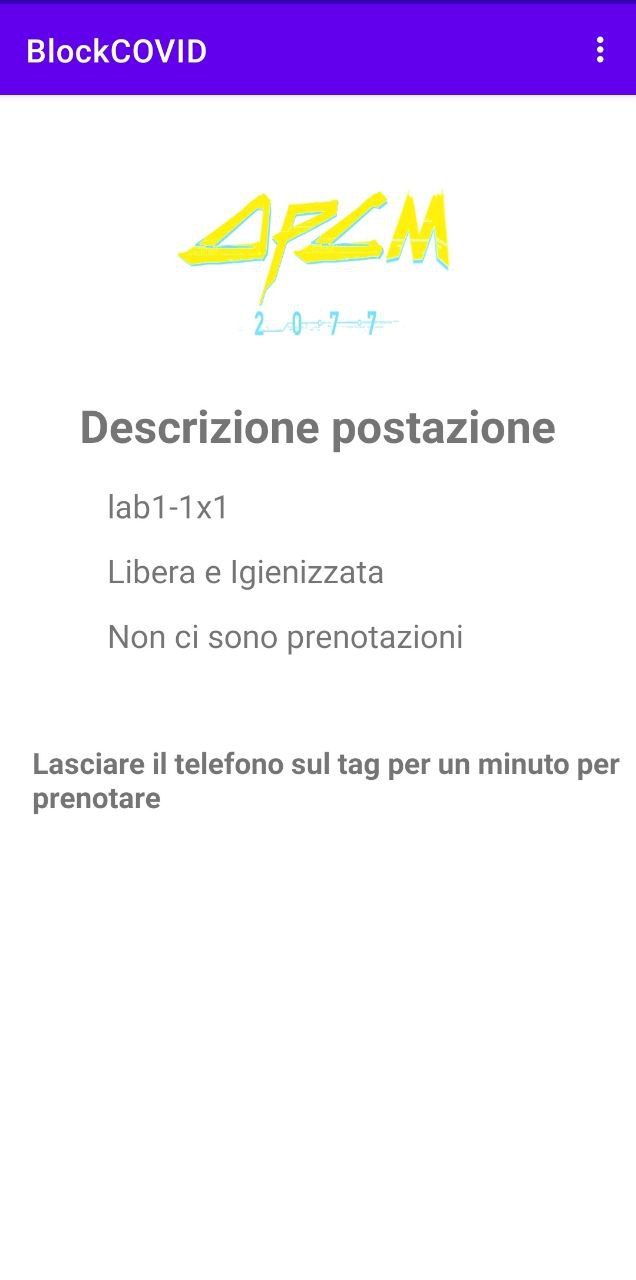
\includegraphics[width=5cm]{res/images/DescrizionePostazione1.png}
	\caption{Stato postazione}
\end{figure}
L'utente ha effettuato la scansione di una postazione e riceve le seguenti informazioni nella pagina principale dell'applicazione:
\begin{itemize}
	\item stanza della prenotazione e posizione indicata tramite x e y;
	\item stato della postazione;
	\item eventuale nome del dipendente che ha prenotato la postazione.
\end{itemize}
 
\subsubsection{Occupazione postazione}
\begin{figure}[H]
	\centering
	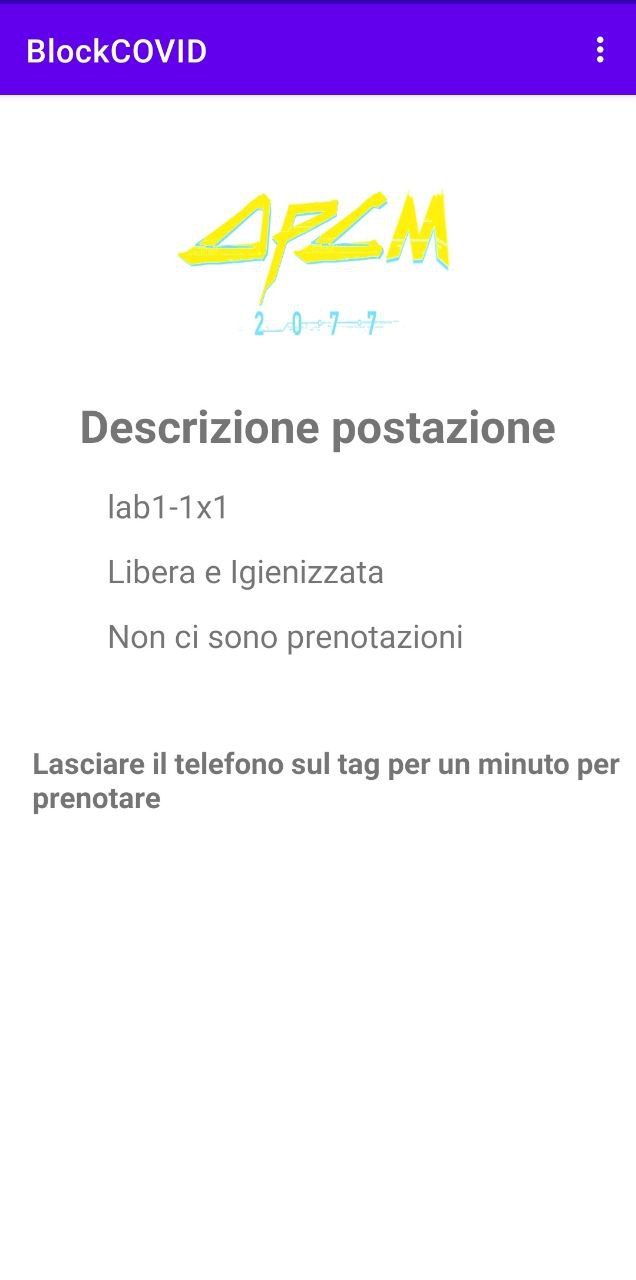
\includegraphics[width=5cm]{res/images/DescrizionePostazione1.png}
	\caption{Inizio occupazione postazione}
\end{figure}
L'utente dopo aver scansionato con il proprio smartphone il tag NFC per
un tempo maggiore o uguale ad un minuto, prenota in modo automatico la postazione per
l’intera giornata lavorativa. Lo stato della postazione deve essere libera e igienizzata e non prenotata da un altro utente durante il resto della giornata.
\subsubsection{Igienizzazione postazione}
\begin{figure}[H]
	\centering
	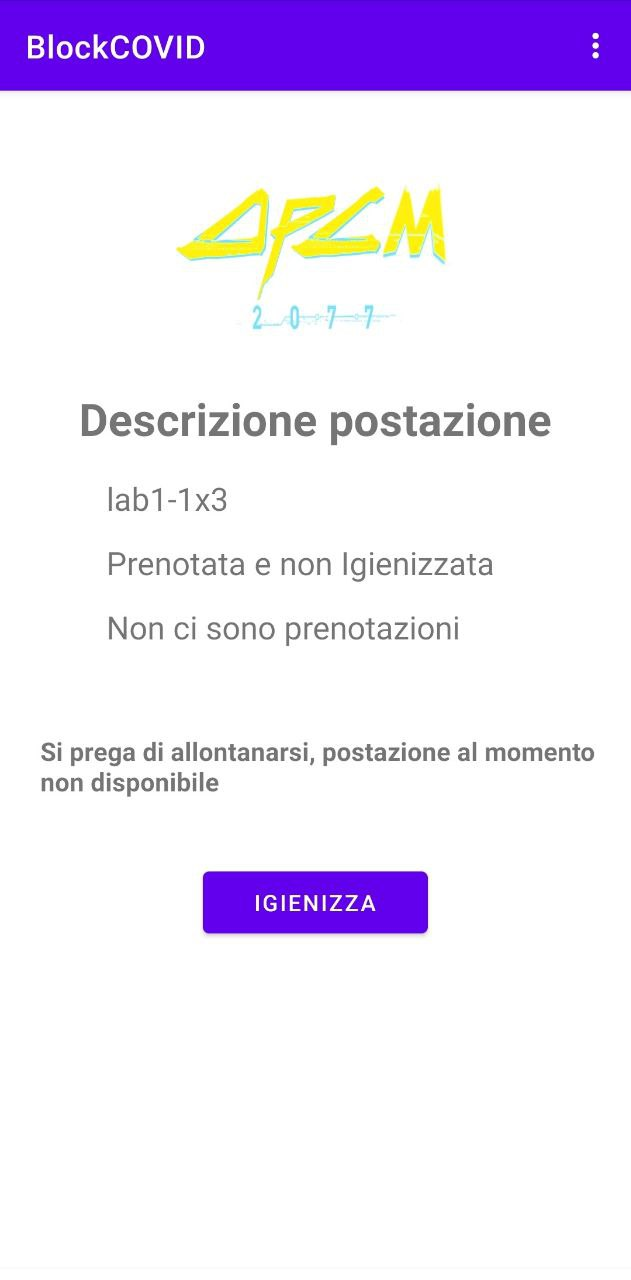
\includegraphics[width=5cm]{res/images/DescrizionePostazione3.png}
	\caption{Igienizzazione postazione}
\end{figure}
L'utente igienizza una postazione il cui stato è diverso da "igienizzato" e lo segnala premendo l'apposito bottone "igienizza" nella pagina principale dell'applicazione. In modo automatico lo stato della postazione viene registrato come libera e igienizzata o prenotata e igienizzata.
\subsubsection{Visualizzazione lista prenotazioni}
\begin{figure}[H]
	\centering
	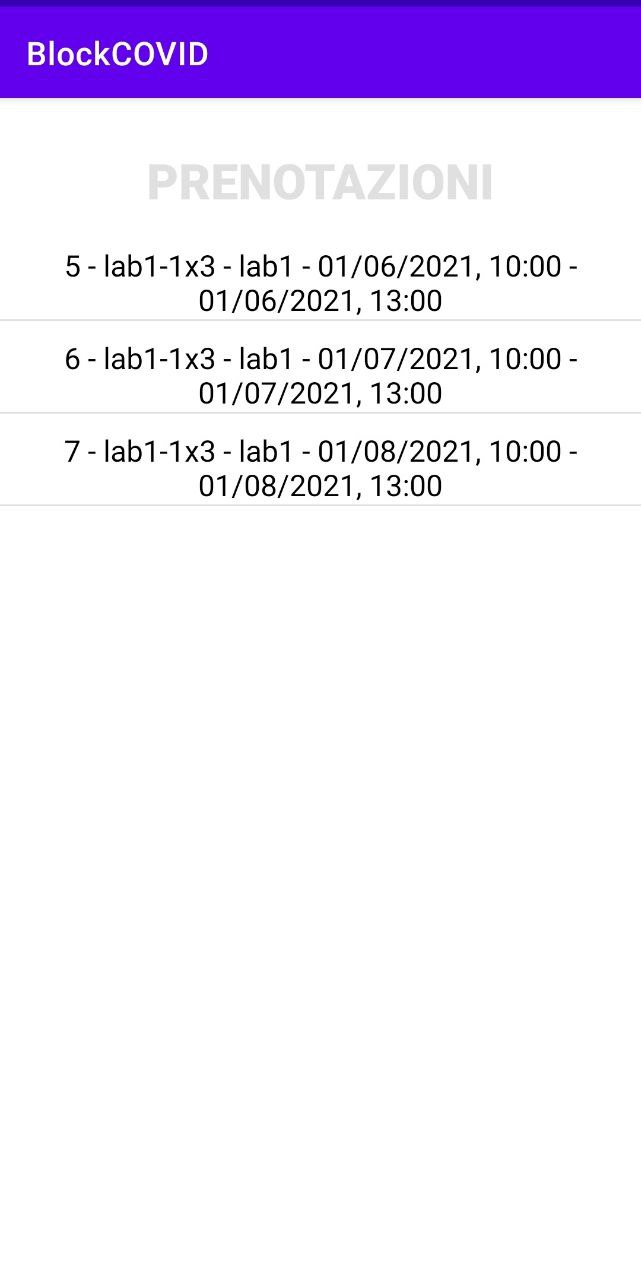
\includegraphics[width=5cm]{res/images/VisualizzaPrenotazioni.png}
	\caption{Visualizzazione lista prenotazioni}
\end{figure}
L’utente può accedere alla sezione per la visualizzazione della lista delle prenotazioni da lui effettuate, cliccando il menù a tendina in alto a destra.
Ogni postazione mostra le seguenti informazioni:
\begin{itemize}
	\item stanza della prenotazione;
	\item posizione indicata tramite x e y;
	\item data di inizio della prenotazione;
	\item orario di inizio della prenotazione;
	\item data di fine della prenotazione;
	\item orario di fine della prenotazione.
\end{itemize}
\subsubsection{Disdetta prenotazione}
\begin{figure}[H]
	\centering
	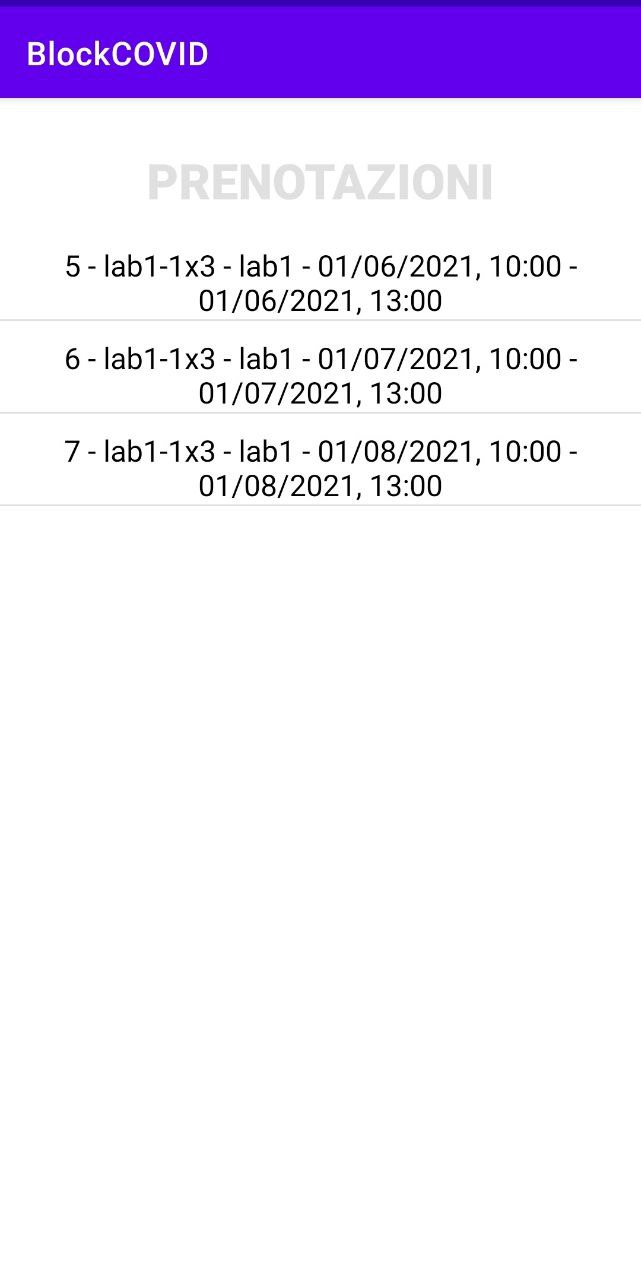
\includegraphics[width=5cm]{res/images/VisualizzaPrenotazioni.png}
	\caption{Disdetta prenotazione}
\end{figure}
L’utente disdice una prenotazione da lui effettuata in precedenza.
\subsubsection{Guida utente}
\begin{figure}[H]
	\centering
	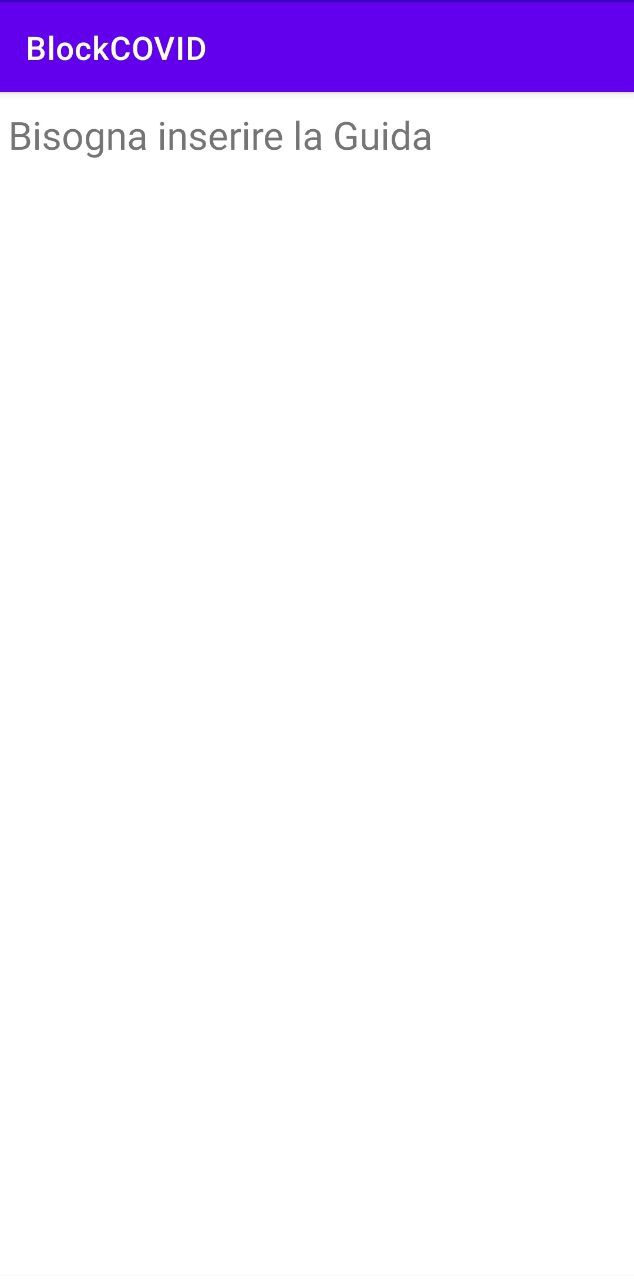
\includegraphics[width=5cm]{res/images/Guida.png}
	\caption{Guida dipendente}
\end{figure}
L’utente riceve una guida riguardo le funzionalità principali dell'applicazione.
\subsubsection{Prenotazione postazione}
\begin{figure}[H]
	\centering
	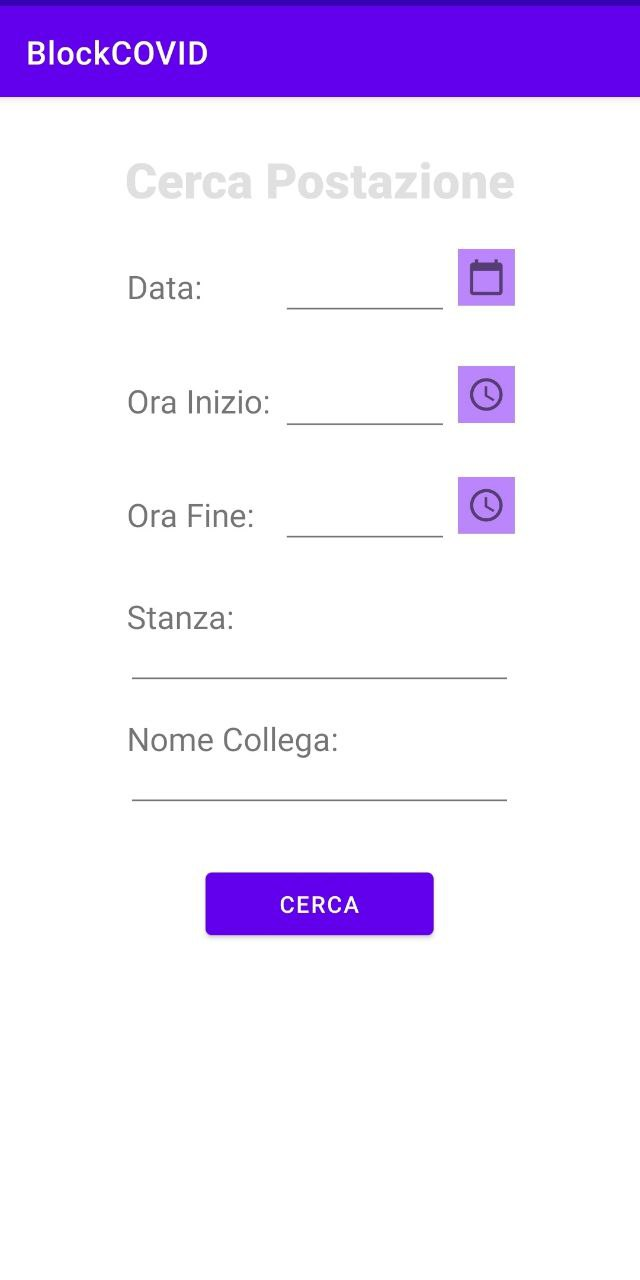
\includegraphics[width=5cm]{res/images/PrenotaPostazione.png}
	\caption{Prenotazione postazione}
\end{figure}
Il dipendente può prenotare una postazione premendo sull'elemento della lista "Prenota postazione" del menù principale in alto a destra.
Dopo aver premuto dovrà inserire la data, l'ora di inizio, l'ora di fine e la stanza obbligatoriamente e in modo facoltativo anche il nome del collega.
Una volta premuto sul bottone "Cerca", se è stato inserito il nome del collega, visualizzerà tutte le sue prenotazioni effettuate nella stanza, nel range orario e nella data inseriti e scorrendo sotto visualizzerà tutte le postazioni di quella stanza con il loro stato e potrà decidere quale prenotare se disponibile. 



\subsection{Addetto alle pulizie}